\section{Theorie}
\label{sec:Theorie}

Unter Diffraktion oder Lichtbeugung versteht sich die Ausbreitung von Licht 
durch Wellen beim Passieren eines Lichtspaltes oder ähnlichen optischen 
Gegenständen. Zur Erklärung dessen kann das Prinzip von Huygens herangezogen 
werden, welches besagt, dass jeder Punkt einer Wellenfront dient als 
Ausgangspunkt einer neuer Elementarwelle durch konstante Aussendung von 
Kugelwellen. Licht kann diffrangieren, wenn das zu passierende Hindernis circa 
in der Größenordnung der Wellenlänge $\lambda$ des ausgestrahlten Lichtes 
liegt. In diesem Experiment soll es um die Fraunhofer Beugung gehen, da ihre 
mathematische Beschreibung simpler ist als die Fresnel Beugung. Das Schema 
der Fraunhofer Beugung ist in \autoref{fig:f1} dargestellt.
\begin{figure}[H]
    \centering
        \centering
        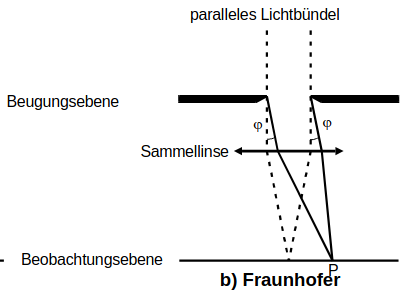
\includegraphics[width=0.6\textwidth]{Bilder/Fraunhoferschema.png}
        \caption{Fraunhofer Beugung. \cite{anleitung3}}
    \hfill
    \label{fig:f1}
\end{figure}
\noindent Licht wird als paralleles Lichtbündel zum Spalt geleitet. Hinter dem
Spalt überlagern sich die ausgesendeten Kugelwellen. Im Winkel $\varphi$ interferieren 
die Wellen und treffen auf die Sammellinse, welche das Fernfeld simulieren soll,
indem sie das Licht in einem Punkt $P$ zusammenführt.
\noindent Das Beugungsobjekt ist ein Spalt, welcher über eine verhältnismäßig
sehr große Länge verfügt. Jenes hat den Zweck, das Experiment auf einer einzigen 
Dimension durchzuführen. Die Welle, welche sich dem Spalt nähert, kann mit 
der Feldstärke
\begin{equation}
    \label{eqn:1}
    A(z,t) = A_0 e^{i\left(\omega t - \frac{2 \pi z}{\lambda}\right)}
\end{equation}
modelliert werden. Den Schwingungszustand eines Puntkes kann durch Überlagerung 
von Elementarwellen, welche gleichzeitig in einem Betrachtungspunkt angelangen,
bestimmt werden. Solche zwei sich überlagernden Wellen, welche um das Stück $x$
versetzt sind, haben durch den Wegunterschied $s$ folglich die Phasendifferenz
\begin{align}
    \label{eqn:2}
    \delta &= \frac{2 \pi s}{\lambda} \\
    \label{eqn:3}
           &= \frac{2 \pi x \sin(\varphi)}{\lambda}.
\end{align}
\noindent Diese wird in der Summation der Strahlenbündel folgendermaßen integriert:
\begin{equation}
    \label{eqn:4}
    B(z,t,\varphi) = A_0 \int_0^b e^{i\left(\omega t - \frac{2 \pi z}{\lambda}
    + \delta\right)} dx
\end{equation}
\noindent Nach der Integration ergibt sich für die Amplitude in $\varphi$-Richtung:
\begin{equation}
    \label{eqn:5}
    B(z,t,\varphi) = A_0 e^{i\left(\omega t - \frac{2 \pi z}{\lambda}\right)}
    \cdot \frac{\lambda}{\pi \sin(\varphi)} e^{\frac{\pi i b \sin(\varphi)}{\lambda}}
    \cdot \frac{1}{2i} \left(e^{\frac{\pi i b \sin(\varphi)}{\lambda}}
    -e^{-\frac{\pi i b \sin(\varphi)}{\lambda}}\right)
\end{equation}
\noindent Unter Einbeziehung der eulerschen Formel lässt sich dieser Ausdruck
wiederum vereinfachen:
\begin{equation}
    \label{eqn:6}
    B(z,t,\varphi) = A_0 e^{i\left(\omega t - \frac{2 \pi z}{\lambda}\right)}
    \cdot e^{\frac{\pi i b \sin(\varphi)}{\lambda}} \cdot \frac{\lambda}{\pi \sin(\varphi)}
    \sin\left(\frac{\pi b \sin(\varphi)}{\lambda}\right)
\end{equation}
\noindent Da das Quadrat der Amplitude proportional zur Intensität ist, ergibt 
sich:
\begin{equation}
    \label{eqn:7}
    I^2 (\varphi) \propto B^2 (\varphi) = A_0^2 b^2 \left(\frac{\lambda}
    {\pi b \sin(\varphi)}\right)^2 \sin^2 \left(\frac{\pi b \sin(\varphi)}
    {\lambda}\right)
\end{equation}
Für den Doppelspalt lässt sich die Intensität gleichermaßen berechnen. Dieser 
soll als Überlagerung zweier Einzelspalte mit Breite $b$ und Abstand $s$ 
installiert sein. Es ergibt sich:
\begin{equation}
    \label{eqn:8}
    I^2 (\varphi) \propto B^2 (\varphi) = 4 \cos^2 \left(\frac{\pi s \sin(\varphi)}
    {\lambda}\right) \cdot \left(\frac{\lambda}{\pi b \sin(\varphi)}\right)^2
    \cdot \sin^2\left(\frac{\pi b \sin(\varphi)}{\lambda}\right)
\end{equation}

\subsection{Fehlerrechnung}
Die gemessenen Werte unterliegen Messunsicherheiten und werden demnach im
Folgenden nicht als fehlerfrei angesehen. Die Fehler entstehen bei der
Bildung der Mittelwerte durch den Fehler des Mittelwerts und bei der
Regressionsrechnung sowie der Fehlerforpflanzung durch Python.
Der Fehler des Mittelwerts ist gegeben durch 
\begin{equation}
    \begin{aligned}
        \increment \overline{x} &= \sqrt{\overline{x^2\kern-0.1em} - \overline{x}^2} \\
                            &= \frac{\sqrt{\frac{1}{N-1} \sum\limits_{i=1}^N (x_i - \overline{x})^2}}{\sqrt{N}}.
    \end{aligned}
\end{equation}

Um Fehler einzubeziehen, wird die Gauß'sche Fehlerfortpflanzung verwendet:
\begin{equation}
    \label{eqn:9}
    \increment f = \sqrt{\left(\frac{\partial f}{\partial x}\right)^2 \cdot \left(\increment x\right)^2 + \left(\frac{\partial f}{\partial y}\right)^2 \cdot \left(\increment y\right)^2 + .... + \left(\frac{\partial f}{\partial z}\right)^2 \cdot \left(\increment z\right)^2}
\end{equation}